\documentclass{article}

\usepackage[english]{babel}

\usepackage[letterpaper,top=2cm,bottom=2cm,left=3cm,right=3cm,marginparwidth=1.75cm]{geometry}

\usepackage{amsmath}
\usepackage{amssymb}
\usepackage{graphicx}
\usepackage{float}
\usepackage{placeins}

\usepackage[colorlinks=true, allcolors=blue]{hyperref}

\title{Design of a Electric Tiller }
%\author{Blessings Mambwe}

\begin{document}
\maketitle

%\begin{abstract}
%Your abstract.
%end{abstract}
\begin{flushleft}
\section{Introduction}
Electric Tillers are used to cultivate land, to prepare it for planting. 
The majority however are powered by internal combution engines which are costly
exhauts poluttans.\\
This has motivated the design of efficient Electric tiller. 


\section*{Agricultural Cultivation Principles}
\subsection*{Soil}
The physics of soil is a complex phenomenon that allows particles to behave like a fluid in terms of movement and solid when enough particles gather in one place. 
Unlike fluids, which can be mathematically represented using the Navier-Stokes equations, the behavior of soil is a complex topic that is still under research.
Characteristics of soil, such as particle size, shape, and texture, influence its hardness and its capacity for transportation (G. Ranjan, 2001). \newline
There are many different kinds of soil, with the most common types being:
\newline


\vspace*{5pt}

\textbf{Clay Soil }: Clay Soil: It is typically brown in appearance and is a fine-textured, grainy soil. 
It has the smallest particle size of 0.002mm or less in diameter. Clay soil is smooth and lumpy, and it dries slowly, becoming very firm. 
While it can store a large amount of water and is rich in minerals, it allows water to travel very slowly, reducing the rate of water drainage. 
For this reason, it is not suitable for farming.
\newline
\vspace*{3pt}

\begin{center}
\begin{figure}[h]
    \centering
%\hspace*{-1.53cm}

\includegraphics[scale=0.5]{Soil/Clay-Soil.jpg}
\caption{Image of clay soil}
\end{figure}
\end{center}

\vspace*{5pt}
 \textbf{Silt Soil}: Silt soil is light, granular, and feels powdery when dry and slippery when wet. It often consists of a mixture of sand and clay.
  It is composed of small to medium-sized particles ranging from 0.002mm to 0.06mm in diameter. Silt soil has a moderate water-holding capacity and maintains a good balance between water drainage and retention. It is also rich in minerals. However, its biggest drawback is that it can easily wash away in the rain. Additionally, it becomes very compact when wet, reducing its aeration.
\newline
\vspace*{3pt}

\begin{center}
\begin{figure}[h]
    \centering
%\hspace*{-1.53cm}

\includegraphics[scale=0.5]{Soil/Silt-Soil.jpg}
\caption{Image of silt soil}
\end{figure}
\end{center}

\textbf{Sand Soil}: This type of soil is light, granular, and feels gritty. It easily flows like a fluid due to its particle size and texture, which range from 0.05mm to 2mm in diameter.
 Sand soil is well-aerated and has good water drainage, allowing for the exchange of gases and atmosphere. However, it has low water-holding capacity due to its particle size, causing water to dry quickly. It is also more susceptible to soil erosion, making it unsuitable for farming.
\newline
\begin{center}
    \begin{figure}[h]
        \centering
    %\hspace*{-1.53cm}
    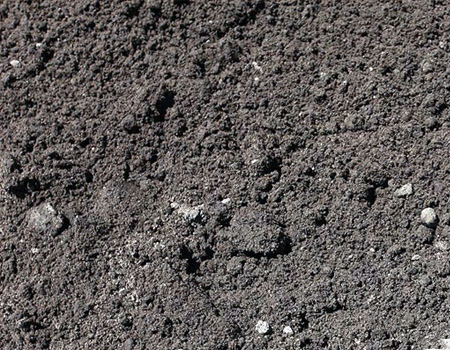
\includegraphics[scale=0.5]{Soil/Sand-Soil.jpg}
    \caption{Image of sand soil}
    \end{figure}
    \end{center}


\vspace*{5pt}
\textbf{Loam Soil}: Loam soil is crumbly and granular, offering a good balance between grittiness and stickiness. It is composed of a mixture of sand, silt, and clay, 
benefiting from the advantages of each soil type. Loam soil is fertile, workable, contains a good amount of nutrients, and allows for optimal root penetration. For these reasons, it is the preferred soil for farming.

Soil preparation is one of the initial steps that a farmer must undertake before engaging in farming. This crucial process involves several steps, including:
\newline

\begin{center}
    \begin{figure}[h]
        \centering
    %\hspace*{-1.53cm}
    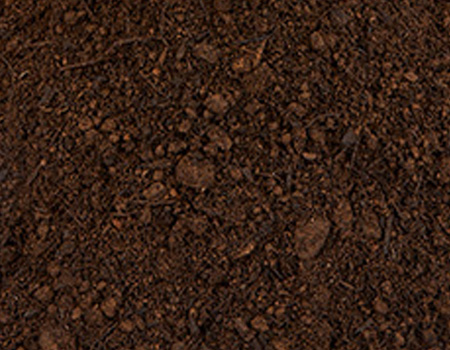
\includegraphics[scale=0.5]{Soil/Loam-Soil.jpg}
    \caption{Image of loam soil}
    \end{figure}
    \end{center}
\vspace*{3pt}

\begin{itemize}
\item \textbf{Testing Soil}: Before planting any crops, it's essential to test the soil to determine its nutrient content, pH levels, and other relevant characteristics. Soil testing helps farmers understand the specific needs of their soil and what amendments may be required.
\newline
\vspace*{3pt}

\item \textbf{Soil Amending}: Based on the results of soil testing, farmers may need to amend the soil to optimize its conditions for plant growth. This can involve adding organic matter (such as compost or manure), adjusting pH levels, and supplementing with necessary nutrients through fertilizers.

\item \textbf{Watering}: Adequate water management is essential for successful crop growth. Farmers need to ensure that the soil has the right moisture content for the specific crops they intend to cultivate. Proper irrigation methods are crucial for maintaining consistent soil moisture.

\item \textbf{Tillage}: Depending on the farming method and crop type, tillage may be necessary. Tillage involves preparing the soil by plowing, cultivating, or otherwise breaking up the ground to create a suitable seedbed. However, conservation tillage practices are increasingly used to minimize soil disruption.
\end{itemize}


\section*{Existing Cultivating Mechanisms}
Tilling is the process of breaking up and loosening soil to prepare it for planting. Various types of machinery can be used.
 To decide on the appropriate machinery, one needs to consider the following factors:
\newline

\textbf{Capacity}: This refers to the amount of work a machine can accomplish per hour on a particular area.
 It can be calculated using the equation:
 \begin{align*}
    C_{a} = \frac{v \cdot w \cdot n_f}{100} 
\end{align*}
\vspace*{2pt}

Where $v$ = travel speed $\frac{km}{h}$ , $w$ = machine working width (m), $n_f$ = field efficiency(int)
$C_a$ = Capacity field Efficiency.
\newline
\vspace*{2pt}

\textbf{Field Efficiency}: This represents the theoretical amount of time required to execute field operations and can be calculated using the formula:

\begin{align*}
T_t = \frac{A}{C_a}
\end{align*}


Where $T_t$ is the time required.
$A$ is the area to be processed.
$C_a$ is the field capacity.
Below are some modern cultivating tools and machinery.

\textbf{power}

\vspace*{5pt}

\textbf{Hoe}: A hoe is a simple and effective tool that is used in domestic and medium-sized environments. The head, which also acts as the pivot, is the working principle of the hoe. It is bladed to increase the amount of pressure so that it can cut through soil effectively. It is connected to the shaft at a 90-degree angle, from which the load is applied.
\newline

\begin{center}
    \begin{figure}[h!]
        \centering
    %\hspace*{-1.53cm}
    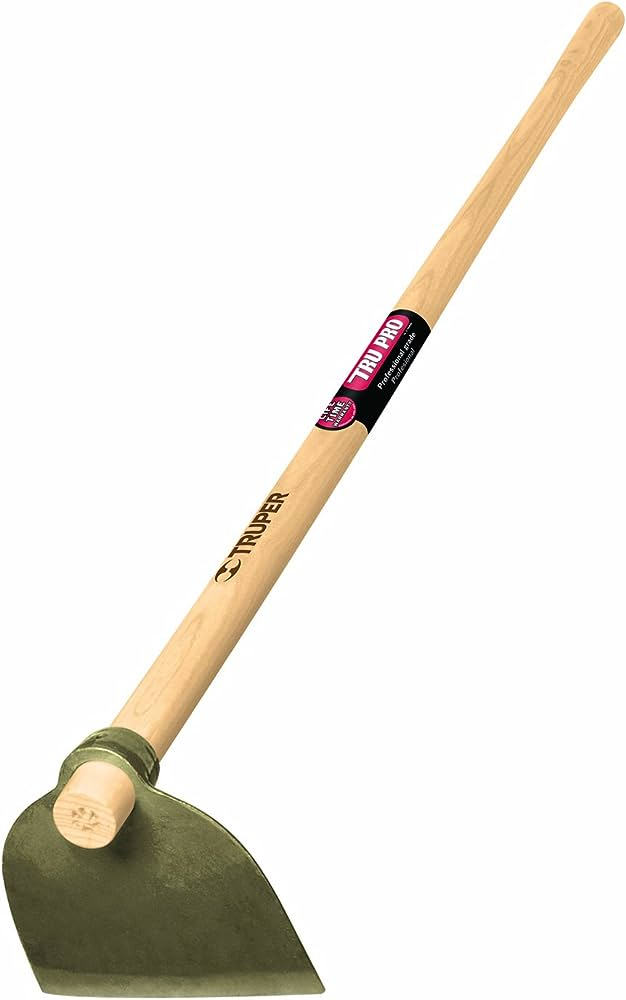
\includegraphics[scale=0.1]{cultivating_tool/hoe.jpg}
    \caption{Hoe}
    \end{figure}
    \end{center}


\vspace*{3pt}
\textbf{Subsoiler}: Also known as a flatlifter or chisel plow, it is a deep soil cultivation tool used for breaking soil at depths of approximately 25 to 50 mm.

Its main components include a shank that penetrates the soil, a blade at the lower end for fracturing and compacting soil layers. Typically, it is mounted onto a tractor, and a control mechanism is adjusted to set the desired depth. Finally, the tractor travels at a steady speed over the working area.
\newline
\FloatBarrier
\begin{center}
    \begin{figure}[htbp]
        \centering
    %\hspace*{-1.53cm}
    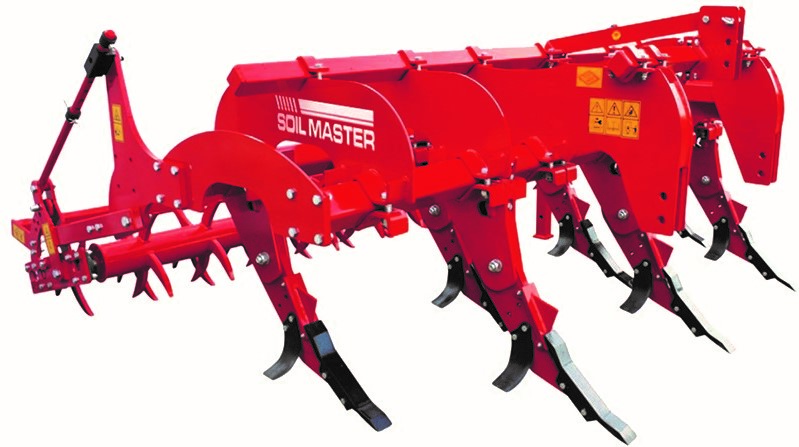
\includegraphics[scale=0.25]{cultivating_tool/subsoiler.jpg}
    \caption{Subsoiler}
    \end{figure}
\end{center}
\FloatBarrier

%\vspace*{3pt}

\subsection*{Non-Electric Tillers}

\textbf{Moldboard Plow}: This equipment dates back to ancient times when it was used to turn sod and prepare fields for crops. It can cut at depths between 15 to 30 inches and is used to cut, lift, and partly turn the soil at an angle during the initial cultivation preparation stage.
\newline 

It consists of the moldboard, a curved metal plate that turns and lifts the soil, and a coulter, which can be a blade or a sharp disk.\newline

Similar to a subsoiler, it is mounted on a tractor, and the plow's depth is adjusted and positioned at an angle to slice through the soil.
\newline
\FloatBarrier
\begin{center}
    \begin{figure}[htbp]
        \centering
    %\hspace*{-1.53cm}
    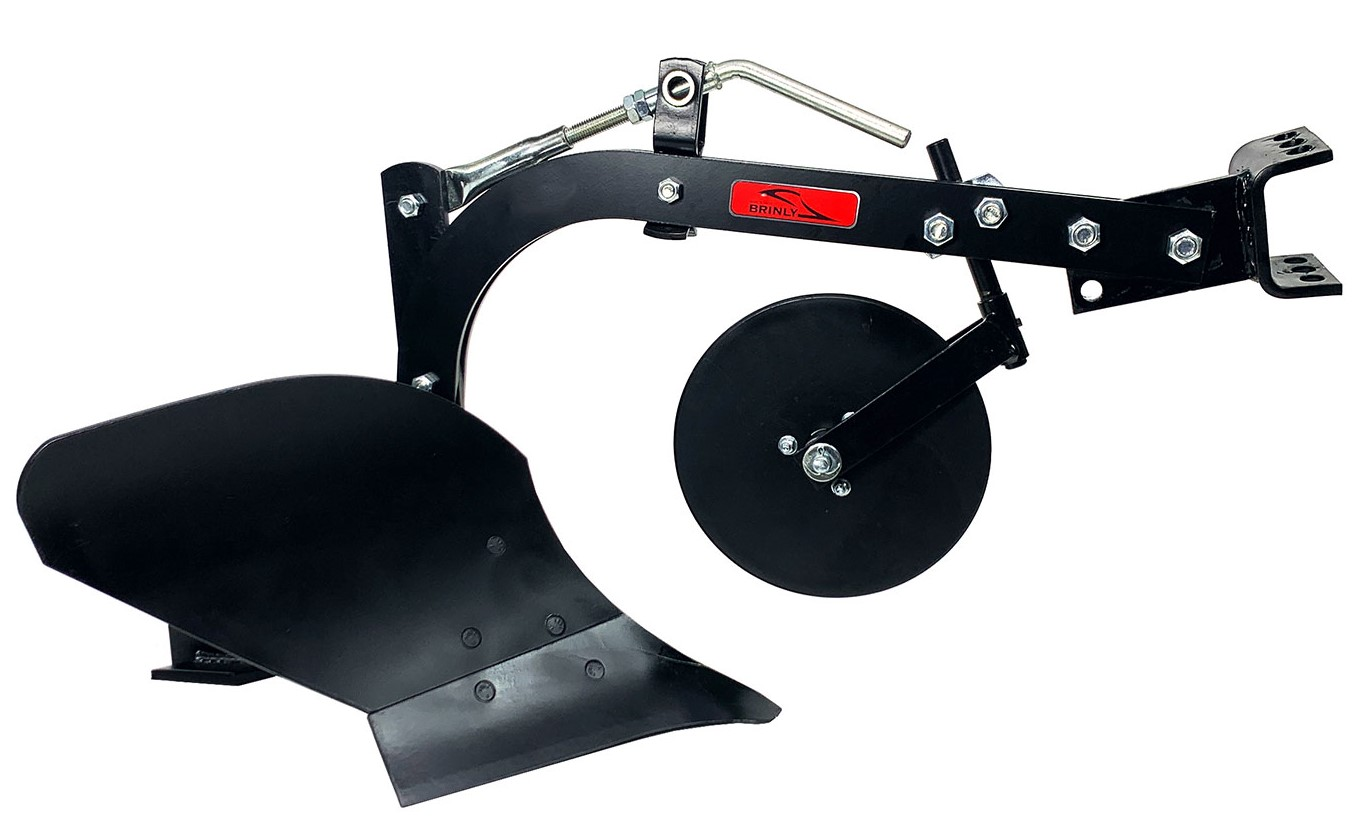
\includegraphics[scale=0.2]{cultivating_tool/moadboadplow.jpg}
    \caption{Moldboard Plow}
    \end{figure}
    \end{center}
\FloatBarrier
\vspace*{3pt}

\textbf{Disc Harrow}: Unlike the tillers mentioned above, the disc harrow is primarily used for secondary tilling to cut out weeds and crop residues. It is also employed for leveling and preparing seedbeds. The depth and operations depend on the specific use; however, it typically cuts within the range of 7.5 cm to 15 cm.\newline

It is composed of circular and concave disc blades mounted on a horizontal shaft. The disc blades are arranged in gangs that are coupled together to till the soil. \newline

The working principle is similar to other machinery; the disc harrow is mounted to a tractor and positioned at an angle along the edge of the field to drive the harrow in vertical overlapping intervals. \newline
\newline 

\FloatBarrier
\begin{center}
    \begin{figure}[htbp!]
        \centering
    %\hspace*{-1.53cm}
    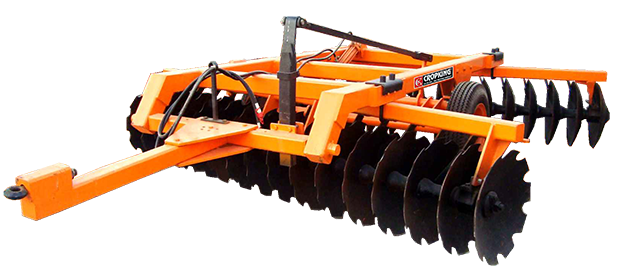
\includegraphics[scale=0.025]{cultivating_tool/disc_harrow.png}
    \caption{Disc Harrow}
    \end{figure}
    \end{center}
    \FloatBarrier
%\vspace*{3pt}

\textbf{Roller-Packer}: Also known as a land presser, cultipacker, or land roller, it is used as a secondary tillage implement, typically in dry seasons, to compact and compress soil after plowing. 
It seals the top millimeters of worked soil and breaks down clods, thereby leveling the land. \newline

Its main component is the heavy roller, which is cylindrical in shape and is often made of steel or cast iron. Attached to the roller are evenly spaced wheels that create pressure points for soil compaction.
\newline
\FloatBarrier
\begin{center}
    \begin{figure}[htbp!]
        \centering
    %\hspace*{-1.53cm}
    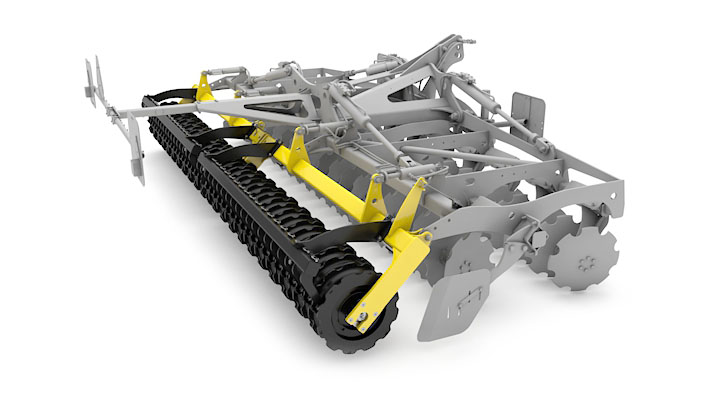
\includegraphics[scale=0.35]{cultivating_tool/roller-packer.jpg }
    \caption{Roller Packer}
    \end{figure}
    \end{center}
\FloatBarrier

\vspace*{3pt}

\textbf{Tractor-Mounted Tiller}: As the name suggests, this implement comprises a frame and rotating blades mounted to a tractor for primary cultivation.
 The depth of cutting can vary according to its design.
 Common uses include seed preparation, leveling, weed control, and soil aeration. \newline

The rotating blades are attached to a horizontal shaft, which is supported by the frame. \newline
Although this type of tiller is versatile and highly efficient, its biggest drawback is the need for fuel consumption and surface disturbance. \newline
\FloatBarrier
\begin{center}
    \begin{figure}[htbp!]
        \centering
    %\hspace*{-1.53cm}
    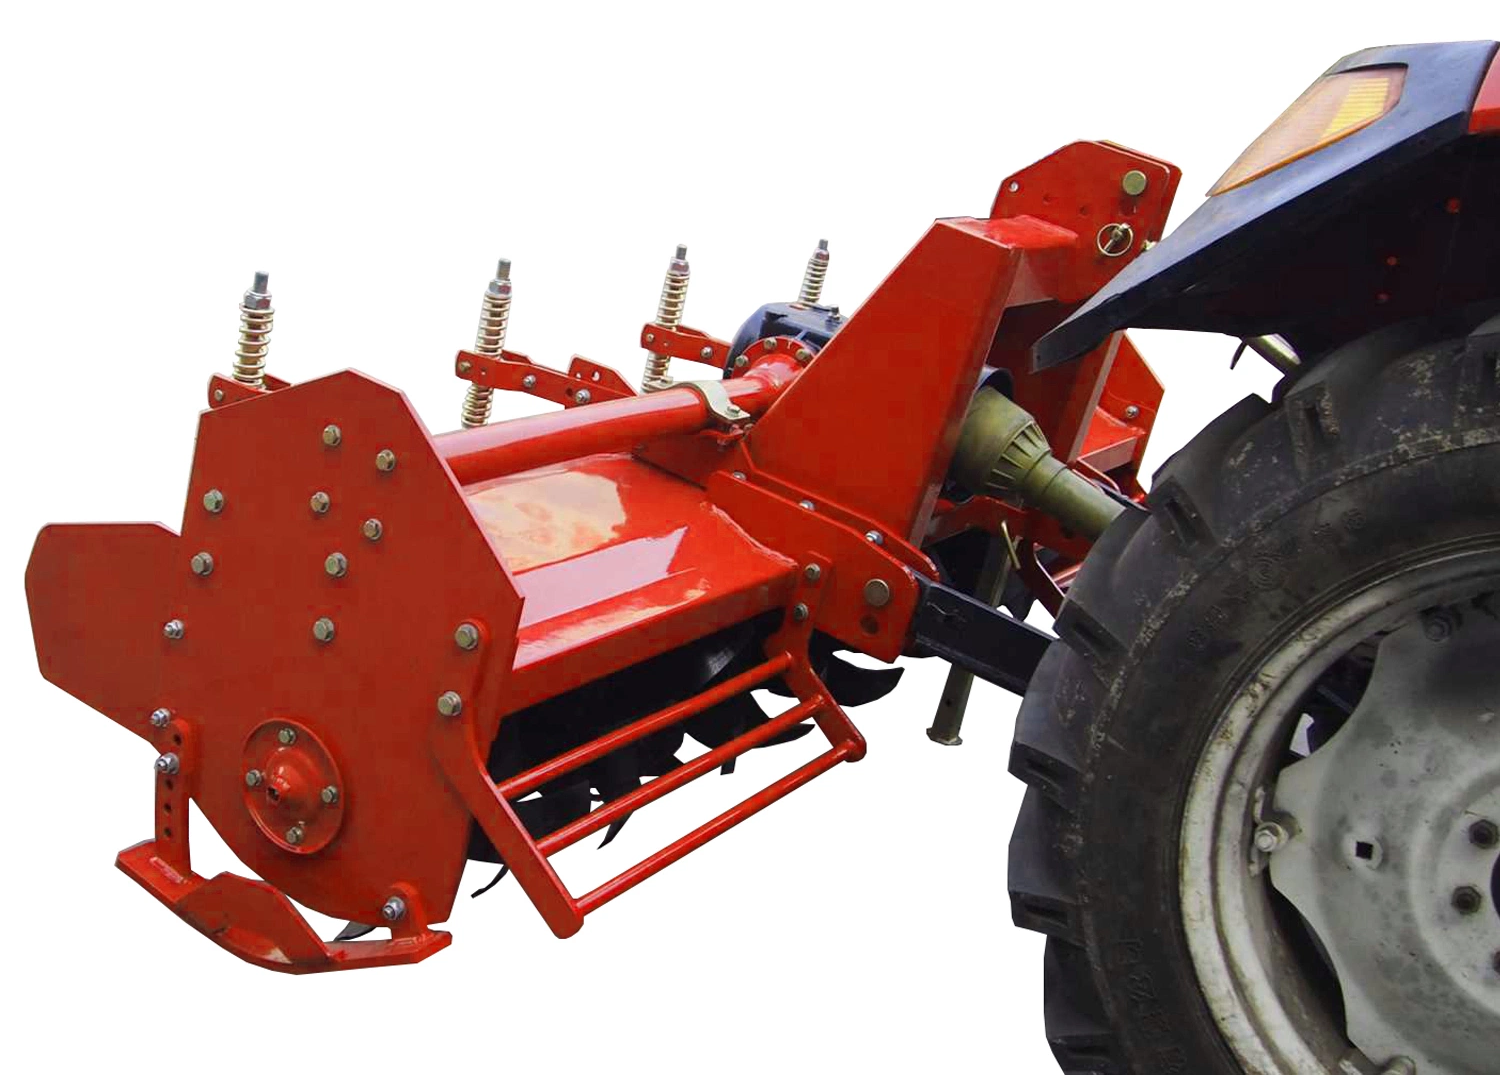
\includegraphics[scale=0.13]{cultivating_tool/Tractor-Mounted-Rotary-Tiller.jpg }
    \caption{Tractor Mounted Tiller}
    \end{figure}
    \end{center}
\FloatBarrier
\subsection*{Commercial Electric Tillers}
\textbf{LawnMaster TE138W1 }
%Image%


\section*{Battery Technology}
\subsection*{Theory}

A battery is a device that converts chemical energy into electrical energy through an electrochemical electrolysis process. \newline

Electricity is nothing more than the flow of electrons in a wire. In direct current (DC), electrons flow in one direction, while in alternating current (AC), electrons alternate back and forth, creating a charge. \newline

The negative electrode is called the anode. This is where oxidation occurs during the discharge phase of the battery. A material such as lithium-carbon releases lithium ions and carbon. \newline

As shown in the equation above, lithium ions are extracted from the anode, which is normally made out of graphite, and move through the solvent to the cathode. \newline

The cathode is the positive electrode where reduction takes place. It is typically made of a metal oxide. For instance, lithium cobalt oxide discharges lithium ions and copper oxide. \newline

\subsection*{Primary Batteries}

Primary batteries are non-rechargeable cells whose electrochemical reactions cannot be reversed. For instance, in alkaline batteries, zinc from the negative electrode discharges hydrogen ions, resulting in the formation of zinc oxide, water, and electrons. 
Meanwhile, manganese dioxide from the positively charged cathode reacts with water to produce negative electrons, ultimately depleting the charge. This process cannot be easily reversed.
\newline
\vspace*{3pt}

\textbf{Zinc Carbon Battery}: These are dry galvanic cells, the oldest type, and were the first to be created in 1866 by George Leclanché. The anode is made from zinc metal, where electrons become positively charged during the oxidation phase. 
The cathode is made of manganese dioxide (MnO\textsubscript{2}) with a small amount of ammonium chloride (NH\textsubscript{4}Cl) electrolyte paste. The manganese dioxide accepts electrons that are released at the anode.

The equations are as follows:

\begin{align*}
    \text{Anode:} & \quad Zn \rightarrow Zn^{2+} + 2e^- \\
    \text{Cathode:} & \quad MnO\textsubscript{2} + H^+ + e^- \rightarrow MnO(OH) \\
    \text{Overall:} & \quad Zn + MnO\textsubscript{2} + NH\textsubscript{4}Cl \rightarrow ZnCl\textsubscript{2} + MnO(OH) + H\textsubscript{2}O
\end{align*}

Zinc reacts with manganese dioxide and ammonium chloride to produce zinc chloride, manganese hydroxide, and water. It's worth noting that the water is given out in the form of vapor. Additionally, the battery has a sealed design, preventing external reactions, and materials can be reabsorbed by the material.
\linebreak
\vspace*{3pt}

\textbf{Mercury Cell}: Mercury batteries, also known as Ruben Mallory, mercuric oxide batteries, or mercuric-oxygen batteries, offer the advantage of a long shelf life and a steady voltage output. They use mercury compounds (Hg) as the cathode and zinc (Zn) at the anode, with potassium hydroxide (KOH) serving as the electrolyte.

They were widely employed in various small and large appliances, including watches, cameras, and calculators.

The chemical equations for the cell reactions are as follows:

\textbf{Anode Reaction:}

\begin{equation*}
    Zn + 2OH^- \rightarrow ZnO + H_2O + 2e^-
\end{equation*}

\textbf{Cathode Reaction:}
\begin{equation*}
    HgO + H_2O + 2e^- \rightarrow Hg + 2OH^-
\end{equation*}

The overall reaction can be summarized as:
\begin{equation*}
    Zn + HgO \rightarrow ZnO + Hg
\end{equation*}

However, it's important to note that mercury cells have been discontinued and are no longer used due to the toxic nature of mercury, which poses environmental and health risks.
\newline
\vspace*{3pt}

\textbf{Alkaline Cell}: As the name implies, it has a pH above 7. Manganese dioxide makes up the cathode, the positive electrode, while the anode, which is negatively charged, is made of zinc metal. There is a separator between the anode and cathode to prevent direct contact while allowing the movement of ions between them. Additionally, the electrolyte is comprised of a potassium hydroxide solution, which serves as a solvent that allows the flow of ions.

The discharge reactions are as follows:

\textbf{Anode Reaction (Oxidation):}
\begin{equation*}
    Zn + 2OH^- \rightarrow ZnO + H_2O + 2e^-
\end{equation*}

\textbf{Cathode Reaction (Reduction):}
\begin{equation*}
    MnO_2 + H_2O + 2e^- \rightarrow Mn_2O_3 + OH^-
\end{equation*}

The overall equation for the cell reaction is:
\begin{equation*}
    Zn + MnO_2 \rightarrow ZnO + Mn_2O_3
\end{equation*}

\subsection*{Secondary Batteries}

Rechargeable batteries are those that can be discharged and recharged multiple times without significant degradation, offering a long-term and sustainable energy storage solution. \newline

Batteries can be connected either in series or parallel. 
In a series connection, the total voltage output is equal to the sum of the individual cell voltages. In contrast, a parallel connection provides the greatest capacity, thereby increasing the current. \newline

Batteries can be classified as either wet or dry. If the electrolyte is in the form of a paste, the cell is considered dry. Conversely, if the electrolyte is a liquid solution, then it is a wet cell
\newline
\vspace*{3pt}

\textbf{Internal Resistance}: This property refers to the electrode's inherent material resistance that opposes the flow of current within the battery, leading to inefficiencies in energy transfer. \newline

\textbf{Shelf Life}: This is the duration for which a battery can retain its charge before it becomes disposable or no longer functional. Longer shelf life is desirable for batteries used in applications where infrequent use is common. \newline

\textbf{State of Charge (SOC)}: SOC is a measure of the percentage of a battery's capacity that has been discharged, expressed as a percentage of its maximum capacity. It provides insight into how much charge remains in the battery at any given time.\newline

\textbf{Cut-off Voltage}: This refers to the minimum allowed voltage at which a battery is considered fully discharged. It's a critical parameter to prevent over-discharging, which can damage batteries and reduce their lifespan. \newline

\textbf{Energy (Ah) / Nominal Capacity (C-rate)}: This parameter represents the battery's energy capacity, typically measured in ampere-hours (Ah). The C-rate indicates the rate at which the battery is charged or discharged relative to its nominal capacity. Higher C-rates allow for faster charging and discharging but may affect the battery's overall performance and lifespan. \newline
\vspace*{3pt}

\textbf{Nickel-Cadmium Cell}: \textbf{Nickel-Cadmium}: Nickel-Cadmium (NiCd) cells are high-power, high-density rechargeable batteries. They can be manufactured in various sizes and capacities, offering a good cycle life and providing a consistent voltage output. NiCd batteries are capable of withstanding high discharge rates and efficient charging, making them suitable for various types of appliances, including emergency lighting and portable electronics. The cathode is composed of nickel oxide (NiOOH), while the anode consists of metallic cadmium (Cd). The commonly used electrolyte is potassium hydroxide (KOH), which facilitates the movement of ions.

The discharge reactions are as follows:

\textbf{At the Anode (Oxidation):}
\begin{equation*}
    Cd + 2OH^- \rightarrow Cd(OH)_2 + 2e^-
\end{equation*}

\textbf{At the Cathode (Reduction):}
\begin{equation*}
    NiOOH + H_2O + e^- \rightarrow Ni(OH)_2 + OH^-
\end{equation*}

The overall combination of these reactions is:
\begin{equation*}
    Cd + NiOOH \rightarrow Cd(OH)_2 + Ni(OH)_2
\end{equation*}

Due to the toxicity of cadmium, which poses health and environmental risks, NiCd batteries have been largely replaced by more environmentally-friendly options such as Lithium-ion (Li-ion) and Nickel-Metal Hydride (NiMH) batteries.
\newline
\vspace*{3pt}

\textbf{Nickel Metal Hydride}: Nickel Metal Hydride (NiMH) batteries represent an improvement over Nickel-Cadmium (NiCd) batteries, offering a good balance between energy density, environmental friendliness, and cost-effectiveness. The cathode is composed of nickel oxyhydroxide (NiOOH), while the anode is made of a metal that's a hydrogen-absorbing alloy, serving as the source of electrons. The electrolyte used is potassium hydroxide (KOH).

The discharge reactions occur as follows:

\textbf{Anode Reaction (Oxidation):}
\begin{equation*}
    MH + OH^- \rightarrow M + H_2O + e^-
\end{equation*}

\textbf{Cathode Reaction (Reduction):}
\begin{equation*}
    NiOOH + H_2O + e^- \rightarrow Ni(OH)_2 + OH^-
\end{equation*}

The overall discharge equation is:
\begin{equation*}
    MH + NiOOH \rightarrow M + Ni(OH)_2
\end{equation*}

The charging reactions are as follows:

\textbf{Anode Reaction (Oxidation):}
\begin{equation*}
    M + H_2O + e^- \rightarrow MH + OH^-
\end{equation*}

\textbf{Cathode Reaction (Reduction):}
\begin{equation*}
    Ni(OH)_2 + OH^- \rightarrow NiOOH + H_2O + e^-
\end{equation*}

These reactions allow for the charging of NiMH batteries.
\newline
\vspace*{3pt}

\textbf{Lithium Ion (Li-ion)}

Lithium Ion (Li-ion) batteries are modern rechargeable batteries that offer the same energy production as lithium-metal (NiMH) batteries but are approximately 20% to 35% lighter in weight. They possess the highest energy density and capacity, making them the most practical choice for various applications.

The electrolyte used in Li-ion batteries is typically lithium salt, the anode is typically composed of graphite, and the cathode consists of lithium metal oxide or phosphate compounds.

The discharge reactions occur as follows:

\textbf{Anode Reaction:}
\begin{equation*}
    LiC_6 \rightarrow C_6 + Li^+ + e^-
\end{equation*}

\textbf{Cathode Reaction:}
\begin{equation*}
    LiCoO_2 + Li^+ + e^- \rightarrow Li_2CoO_2
\end{equation*}

These reactions facilitate the discharge of Li-ion batteries, providing power for various applications.
\newline
\vspace*{3pt}

\textbf{Lithium Iron Phosphate (LiFePO4)}

Lithium Iron Phosphate (LiFePO4), also known as LFP batteries, offer distinct advantages over traditional lithium-ion batteries. They are renowned for their high energy density, extended cycle life, and remarkable safety features, primarily due to their stable chemical reactions that prevent overheating or fire hazards.\newline

LiFePO4 batteries find valuable applications in various fields, including: 

 \textit{Electric Vehicles (EVs)}: LiFePO4 batteries power electric vehicles, providing reliable energy storage and a longer cycle life compared to conventional lithium-ion batteries.
\newline
\vspace*{1.5pt}

\textit{Renewable Energy }: They are employed in renewable energy systems, such as solar setups and wind energy storage, as an efficient and durable energy storage solution.
\vspace*{1.5pt}

\textit{Portable Electronics}: LiFePO4 batteries are used in portable electronic devices, ensuring a safe and long-lasting power source for everyday use.
\newline
\vspace*{1.5pt}

The chemical reactions within LiFePO4 batteries contribute to their performance and safety:
\newline

\textit{Discharge Reaction (Power Generation)}:
At the anode (discharge), lithium ions (Li+) are released from the anode material (usually graphite) and migrate to the cathode. Simultaneously, electrons are generated at the anode:
\begin{equation*}
    C + LiFePO_4 \rightarrow Li_xC_6 + LiFePO_4
\end{equation*}

\textit{Charge Reaction (Recharging):}
At the cathode (charge), lithium ions (Li+) are received from the anode and stored in the cathode material (LiFePO4). During this process, electrons are consumed at the cathode:
\begin{equation*}
    Li_xC_6 + LiFePO_4 \rightarrow C + LiFePO_4
\end{equation*}

These reactions involve the movement of lithium ions (Li+) between the anode and cathode, facilitating the release and storage of electrical energy. 
The anode is typically made of carbon, such as graphite, which produces lithium ions during discharge.
The cathode consists of lithium iron phosphate (LiFePO4), and a separator and electrolyte made of salt are integral components of LiFePO4 batteries, ensuring their safe and efficient operation.

LiFePO4 batteries have become a preferred choice for applications that demand a high level of safety, reliability, and performance while also prioritizing environmental sustainability.



\section*{Motors}
\subsection*{Theory}
As industries increasingly prioritize sustainability, electric motors have gained favor over traditional engines due to their efficiency and ease of maintenance. \newline
The discovery of electric motors can be attributed to pioneers such as Zenobe Gramme, who stumbled upon the concept accidentally. Gramme's inadvertent connection of an AC generator to a battery resulted in a fascinating phenomenon—rotation. This serendipitous event sparked curiosity and further exploration. \newline

Another significant contributor to the understanding and development of electric motors was Michael Faraday. Through extensive experimentation and research, Faraday provided valuable insights that contributed to both the theoretical foundations and practical designs of electric motors. \newline

Electric motors serve as remarkable devices that transform electrical energy into mechanical energy. They can be categorized into two primary types: DC Motors and AC Motors.\newline

DC Motors, or Direct Current Motors, operate on a continuous flow of electric current, resulting in consistent rotational motion. AC Motors, or Alternating Current Motors, derive their power from periodically changing electric currents, leading to versatile applications and capabilities. \newline

The physics behind electric motors involves the interaction between magnetic fields and electric currents. This interplay generates the mechanical force needed for motion. Understanding this fundamental principle is essential to comprehend the inner workings of these indispensable machines.\newline


\textbf{Permanent Magnet Motors} 

Sometimes called Brushed DC motors, they provide the most simplified DC motor design where magnetic fields are solely provided by permanent magnets. The rotor is wound and connected to a circuit to create an opposing magnetic field to the stationary permanent magnets.

% \begin{equation*}
%     [equations]
% \end{equation*}

% \begin{figure}[h]
%     \centering
%     \includegraphics[width=0.6\linewidth]{motor_design.png}
%     \caption{Motor Design}
% \end{figure}

% \begin{equation*}
%     [electric circuits]
% \end{equation*}

The speed can be increased by increasing armature voltage, which boosts the back electromotive force. However, this would result in a reduction of torque, as the two are inversely proportional to the applied voltage.
\newline
\vspace*{3pt}

Reverse motion can be triggered by changing the polarity of the armature voltage, resulting in a change in current flow, or by using external switching devices.

The permanent magnets are normally made from neodymium-iron-boron (NdFeB) or samarium-cobalt (SmCo), eliminating the need for external field windings.

The brushed design of the motors allows the reversal of current flow, enabling bidirectional motion of the motor. Additionally, the absence of field windings allows for high efficiency.

Furthermore, the simplicity of the design results in a low weight. These advantages make them suitable for use in hybrid electric vehicles, robotics and automation, fans and blowers, and small household appliances.
\newline
\vspace*{3pt}

\textbf{Shunt Motor:} A Shunt Motor is a type of self-excited motor in which the configuration of the rotor and stator are connected in parallel. It can be wound using an armature with a wave winding, where the armature coils are interconnected with each other. This winding is typically used in settings where the machine has high voltage capacity and low current capacity.\newline

Alternatively, it can be configured using lap winding, where the number of parallel paths is equivalent to the number of poles. This winding is typically used in settings where the current capacity of the machine is high, and the voltage capacity is low.\newline

The armature current equation is given by: \newline

\begin{equation*}
    V = I_a \cdot R_a + E_b
\end{equation*}
\begin{equation*}
    E_b = k \cdot \phi \cdot \omega
\end{equation*}

% \begin{figure}[h]
%     \centering
%     \includegraphics[width=0.6\linewidth]{dc_motor_configuration.png}
%     \caption{DC Motor Practical Configuration}
% \end{figure}

% \begin{figure}[h]
%     \centering
%     \includegraphics[width=0.6\linewidth]{lap_vs_wave_winding.png}
%     \caption{Lap Winding vs. Wave Winding}
% \end{figure}

The shunt motor can also be configured using field winding. \newline

Due to the armature's resistance voltage drop, torque has an inverse relationship with speed; it reduces over time as speed increases. \newline

Shunt motors are normally classified as constant-speed motors. They are used in industries where precise control of speed and torque is required. For instance, they are employed in lifts, centrifugal pumps, lathe machines, and fans. \newline
\vspace*{3pt}


\textbf{Separated Excited DC Motors:} As the name implies, this is a type of DC motor where, instead of permanent magnets, a separate voltage source is used to provide magnetic fields through a field winding. The motor is also connected to a separate voltage source to complete the circuit.

The armature current equation is given by:
\[ V = I_a \cdot R_a + E_b \]

Where:
\( V \) - Voltage applied to the motor.
\( I_a \) - Armature current.
\( R_a \) - Armature resistance.
\( E_b \) - Electromotive force (EMF) from the motor.

The back EMF is the voltage generated due to its angular speed.

Torque is determined by the motor's geometry, flux, and current and can be expressed as:
\[ T = K \cdot \phi \cdot I_a \]

Using Faraday's law, we have:
\[ e = K \cdot \phi \cdot \omega \]

Applying Kirchhoff's voltage law:
\[ e = i_a \cdot R_a + L_a \frac{di_a}{dt} + e_b \]

% \begin{figure}[h]
%     \centering
%     \includegraphics[width=0.6\linewidth]{separately_excited_motor_circuit.png}
%     \caption{Circuit Diagram of Separately Excited DC Motor}
% \end{figure}

Separately excited DC motors operate in stable conditions with any excited field, allowing for a wide range of output voltage. This versatility makes them suitable for applications where precise control over voltage and speed is necessary. However, providing an external power supply for these motors can be challenging, and adjusting the field flux to control motor behavior is a complex process that may require sophisticated control systems.
\newline
\vspace*{3pt}

\textbf{Separately Excited DC Motors:} As the name implies, these are a type of DC motor where, instead of permanent magnets, a separate voltage source is used to provide magnetic fields through a field winding. The motor is also connected to a separate voltage source to complete the circuit.

The key equations for this motor include:
\begin{align*}
V &= I_a \cdot R_a + E_b \\
E_b &= K \cdot \phi \cdot \omega
\end{align*}

Where:
$V$ = Applied voltage,
$I_a$ = Armature current,
$R_a$ = Armature resistance,
$E_b$ = Back electromotive force ,
$K$ = Motor constant,
$\phi$ = Flux,
$\omega$ = Angular speed,
$L_a$ = Armature inductance
\newline
\vspace*{3pt}

The back electromotive force ($E_b$) is generated due to the motor's angular speed. The torque ($T$) is a constant depending on the motor's geometry, flux, and current, given by $T = K \cdot \phi \cdot I_a$. 

By applying Faraday's law and Kirchhoff's voltage law, we can see that torque can be controlled by altering the armature voltage, as it is directly proportional to the motor's torque. This allows for precise control of torque. Similarly, current, used to provide the magnetic field, can also be adjusted to increase speed and torque.
\newline
Field flux is inversely proportional to the back electromotive force ($E_b$) from the armature windings, which is directly proportional to the armature speed and flux product. Therefore, an increase in speed results in a reduction of armature voltage, armature speed, and torque. Voltage, current, and flux can be altered to increase or reduce speed and torque.
\newline

Separately excited DC motors offer several advantages, including stable operation with any excited field, allowing for a wide range of output voltages. However, a disadvantage is that providing an external power supply can be challenging, and the ability to alter flux is complex.
\vspace*{5pt}

\textbf{Series DC Motors:} As the name implies, this is a type of DC motor with a configuration where a single voltage supply is connected in series to both the armature winding ($R_a$) and the field winding to provide magnetic fields. Commutators and brushes are used to maintain electrical contact with the rotor.

% \begin{figure}[h]
%     \centering
%     % Insert the image of the electric circuit here
%     \caption{Electric circuit diagram}
% \end{figure}

This motor can generate high torque at low speeds and low torque at high speeds, making it suitable for various applications, including vehicles. The field flux is directly proportional to the armature current, which can be regulated using a diverter to control torque easily. Additionally, resistors can be connected to the field windings to diversify high current.

The series connection of the armature and field windings allows the motor to start with high torque. As a result, they are used in trains, trams, cranes, hoists, and forklifts where critical starting torque is required.
\newline
\\

Since the armature current of the motor depends on the load, the motor should be started without a load to avoid potential damage. While this may initially seem like a disadvantage, the motor's ability to vary its speed and torque depending on the load finds tremendous applications. Specifically, they are used in roller coasters and ferris wheels to create exciting dynamics for amusement park riders. Drill presses exert increasing force on the load, and as the load increases, the speed and torque can be adjusted according to the type of material and load being processed. Other applications include irrigation pumps and conveyor belts. Additional advantages of using DC motors include ease of maintenance, assembly, and design, as well as low cost.
\newline
\\
 Unfortunately, if the load is too high, the armature current increases, resulting in a decrease in speed. They are also not well-suited for high-speed applications due to their inherent design and the relationship with field flux, speed, and back electromotive force (EMF). Moreover, due to the interaction of back EMF and armature current, the motor can only be used for unidirectional applications unless further electrical control is established. Finally, cooling mechanisms such as fans are required to prevent the motor from overheating at low loads due to the high field windings.
\newline
 \vspace*{3pt}

\textbf{Compound DC Motor:} This is another self-excited motor that inherits its configuration from both the shunt motor and the series motor, thereby gaining superior advantages. In this motor, the armature windings are connected in series, while the field winding is in shunt or parallel connections. \newline

% \begin{figure}[h]
%     \centering
%     % Insert the circuit diagram here
%     \caption{Circuit diagram}
% \end{figure}

Compound DC motors combine the superior advantages of both shunt motors and series motors. They can be tailored to specific applications, adopting characteristics from both shunt and series motors. However, building them can be challenging, as winding makes for a complex design. Additionally, controlling speed and torque can be more challenging. \newline

Overall, compound DC motors can be used in settings where both shunt and series motors find application, such as elevators, lifts, electric trains and trams, conveyors, and more. \newline
\newline
 \vspace*{3pt}

 \textbf{Brushless DC Motors/Electronically Commutated Motor:} These are brushless motors that use an electronic controller to excite the windings in the rotor. This excitation causes the magnetic fields to infinitely attempt to align with the polarity of the windings, thus producing motion.

 \begin{figure}[h]
     \centering
     % Insert the motor design image here
     \caption{Motor design}
 \end{figure}
 
 Through an electronic controller, the windings are turned on and off, resulting in the attraction that drives the motor.
 
 The absence of brushes eliminates friction, resulting in greater efficiency. Additionally, they require minimal to no maintenance. Some brushless motors can also be designed for regenerative braking, allowing kinetic energy to be converted back into electric energy during deceleration.
 
 One of the most significant characteristics is their high power-to-weight ratio. For this reason, they are used in various industries, including aerospace for drones to generate lift, marine applications for underwater drones and boats, the medical industry for quiet operation, and the manufacturing industry where they can be employed in flammable environments.
 \newline
 \vspace*{3pt}
 
 \textbf{Induction AC Motors:} Also referred to as asynchronous motors, these motors operate through electromagnetic induction. The stator's winding generates a magnetic field, inducing eddy currents in the rotor, which features a short-circuited winding. Alternating current creates a revolving flux that opposes the rotor's flux, causing the rotor to try to catch up with the stator's rotating magnetic field. This can be single-phase, two-phase, or three-phase alternating current. The slip, defined as the difference between the stator's synchronous speed and the actual rotor speed, is given by the formula:
\[ \text{Slip} = \frac{{N_s - N_r}}{{N_s}} \]

where \( N_s \) is the synchronous speed and \( N_r \) is the rotor's speed.

The rotor of the motor can be designed using a squirrel cage, which includes a cylindrical core with slots twisted at an angle to prevent magnetic locking and maximize slip. Alternatively, they can be designed using a wound rotor, also known as a slip ring. This design includes a laminated cylindrical core with slots on the outer periphery and insulated windings in the rotor arranged uniformly or in star connections. \newline

Induction motors have a simple and rugged design, are cost-effective, and require minimal maintenance. They don't need additional starting motors. Since only the stator is connected to the circuit, electromagnetic flux can be varied by adjusting the voltage, which, in turn, varies the torque linearly. Speed can be adjusted by altering the frequency of the AC power. This can be achieved using variable frequency drives, frequency converters, frequency generators, or motor-generator sets. \newline

Thanks to their high torque, they are used in various industrial applications to drive pumps, compressors, and conveyors. They are also commonly found in HVAC systems for ventilation and air conditioning. Furthermore, they serve as traction motors in electric traction for trains and electric vehicles. \newline

\end{flushleft}

\end{document}